\documentclass{article}
\usepackage{graphicx}
\usepackage{amsmath}
\usepackage{enumitem}
\usepackage{float}
\usepackage{listings}
\usepackage{xcolor}
\usepackage[a4paper, margin=1in]{geometry}
\title{Homework 1}
\author{Steve Gillet}
\date{\today}

% Custom information
\newcommand{\className}{Course: Automatic Control Systems – ASEN 5114-001 – Spring 2025}
\newcommand{\professorName}{Professor: Dale Lawrence}
\newcommand{\taName}{Teaching Assistant: Anantha Dhruva}

\lstdefinestyle{matlabstyle}{
    language=Matlab,              % Specify the language
    basicstyle=\ttfamily\footnotesize\color{black}, % Code font
    keywordstyle=\color{blue}\bfseries, % Keywords in blue
    stringstyle=\color{green},    % Strings in green
    commentstyle=\color{magenta}, % Comments in magenta
    numbers=left,                 % Line numbers on the left
    numberstyle=\tiny\color{black},% Line number style
    stepnumber=1,                 % Line number increment
    breaklines=true,              % Line breaking
    frame=single,                 % Border around code
    backgroundcolor=\color{white},
    tabsize=4,                    % Tab size
    showstringspaces=false,       % Don't show spaces in strings
}

\begin{document}

\maketitle
\textit{
    "Due: Monday, February 3, 2025 at 11:59 pm on Canvas. Please assemble a single PDF file for
    submission that includes your Matlab/Simulink code/diagrams, plots, and explanations of your
    work and the results. Label sections to correspond with those in the assignment. Don’t make it
    difficult to locate the text/code/plots for each section."
}

\section*{1.}

\textit{
    "[10pts] Find the parameters $R_M$, $L_M$, $K_\tau$, $J_M$, and $K_B$ from the motor specification sheet, noting
    units. Also, find the total gear ratio N from the motor shaft to the load shaft, and estimate the
    load shaft moment of inertia $J_L$. Use these to quantify the parameters in the transfer function
    relating $V_P$ to $\Theta_L$. Also, estimate the potentiometer scale factor $K_S$ from the data file posted on Canvas."
}

\begin{figure}[H]
    \centering
    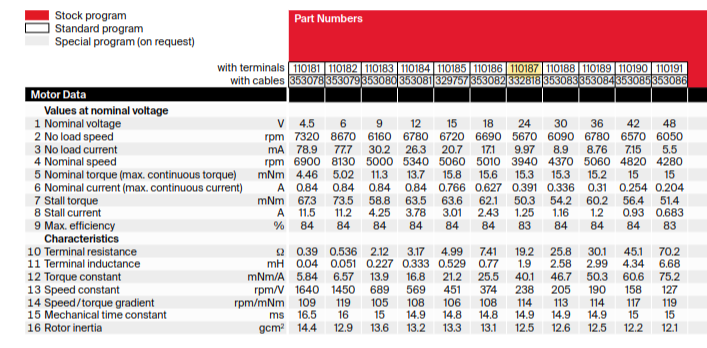
\includegraphics[width=0.9\textwidth]{motorSpec.png}
\end{figure}

I took the parameters from the motor specification table above using part number 110187.
\begin{align*}
    R_M&=19.2\;\Omega \\
    L_M&=1.9\text{mH}=0.0019\text{ H} \\
    K_\tau&=40.1\text{mNm/A}=0.0401\text{ Nm/A}  \\
    J_M&=12.5\text{gcm}^2=0.00000125\text{ kgm}^2 \\
    K_B&=238\text{rpm/V}=0.04\text{ Vs/rad} \\
    N&=3.3 \\
    J_L&=0.018522\text{ kgm}^2 \\
    K_S&=0.8\text{ V/rad}
\end{align*}

I derived N by using the logic that the gear ratio measured in radii is equal to the gear ratio measured in circumferences and if the teeth on both gears are the same size then you could measure the circumference in number of teeth and take the ratio of numbers of teeth.
The load shaft gear has 120 teeth and the motor shaft gear has 36, making the ratio 3.33.

I estimated $J_L$, using standard inertia formulas for a rod rotating about one end and a satellite (for the weight) and added them together.
\\
Equation for rod:
$J_{\text{arm}} = \frac{1}{3} m_{\text{arm}} L^2$
\\
Equation for weight:
$J_{\text{weight}} = m_{\text{weight}} L^2$
\\
\\
I got the mass of the arm and weight using their measurements and the average density for aluminum and brass.
\begin{itemize}
    \item Arm Dimensions: \( L = 30 \) cm, \( h = 0.7 \) cm, \( w = 1.1 \) cm
    \item Volume:
    \begin{equation}
        V_{\text{arm}} = L \times h \times w = 30 \times 0.7 \times 1.1 = 23.1 \text{ cm}^3
    \end{equation}
    \item Density of aluminum: \( \rho_{\text{Al}} \approx 2.7 \) g/cm³
    \item Mass of the arm:
    \begin{equation}
        m_{\text{arm}} = V_{\text{arm}} \times \rho_{\text{Al}} = 23.1 \times 2.7 = 62.37 \text{ g} = 0.0624 \text{ kg}
    \end{equation}
\end{itemize}

\begin{itemize}
    \item Weight Dimensions: \( 3.2 \times 2.0 \times 3.4 \) cm
    \item Volume:
    \begin{equation}
        V_{\text{brass}} = 3.2 \times 2.0 \times 3.4 = 21.76 \text{ cm}^3
    \end{equation}
    \item Density of brass: \( \rho_{\text{brass}} \approx 8.5 \) g/cm³
    \item Mass of the brass weight:
    \begin{equation}
        m_{\text{brass}} = V_{\text{brass}} \times \rho_{\text{brass}} = 21.76 \times 8.5 = 184.96 \text{ g} = 0.185 \text{ kg}
    \end{equation}
\end{itemize}

Then I used those numbers (including length of arm for L) to calculate the moments of inertia and combine them.

\begin{equation}
    J_{\text{arm}} = \frac{1}{3} m_{\text{arm}} L^2
\end{equation}

\begin{equation}
    J_{\text{arm}} = \frac{1}{3} (0.0624) (0.30)^2 = 0.001872 \text{ kg}\text{m}^2
\end{equation}

\begin{equation}
    J_{\text{weight}} = m_{\text{weight}} L^2
\end{equation}

\begin{equation}
    J_{\text{weight}} = (0.185) (0.30)^2 = 0.01665 \text{ kg}\text{m}^2
\end{equation}

\begin{equation}
    J_L = J_{\text{arm}} + J_{\text{brass}}
\end{equation}

\begin{equation}
    J_L = 0.00187 + 0.01645 = 0.018522 \text{ kg}\text{m}^2
\end{equation}

\begin{figure}[H]
    \centering
    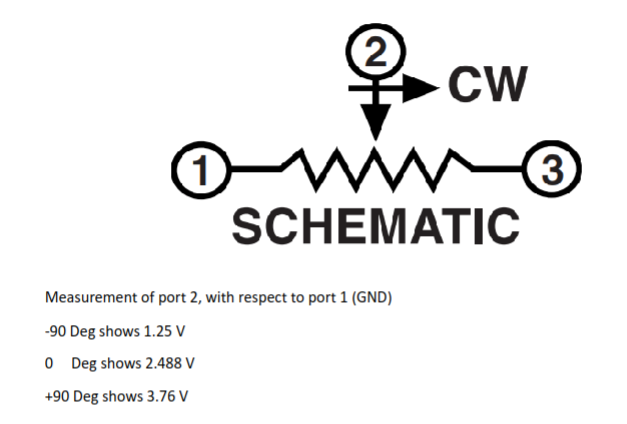
\includegraphics[width=0.8\textwidth]{potentiometerSpec.png}
\end{figure}

To derive $K_S$ I used the readings/schematic above.
I took the total voltage difference over the total angle difference (converted to radians).
\begin{align}
    K_S&=(3.76V-1.25V)/(\frac{\pi}{2}\text{rad}+\frac{\pi}{2}\text{rad}) \\
    K_S&=0.8\text{ V/rad}
\end{align}

The transfer function that relates $V_P$ to $\Theta_L$ is:
\begin{equation}
    \frac{-1}{\frac{1}{NK_{\tau}}J_{eq}L_Ms^3 + \frac{1}{NK_{\tau}}J_{eq}R_Ms^2+NK_Bs}
\end{equation} 

I derived $J_{eq}$ using:

\begin{align*}
    J_{eq} &= J_L + N^2J_M \\
    J_{eq} &= 0.018535612kgm^2
\end{align*}

Plugging in the parameter values:
\begin{equation}
    \frac{-1}{0.000266135\;V\cdot sec^3 \;s^3 + 2.6893656\;V\cdot sec^2\;s^2+0.132\;\frac{V\cdot sec}{rad}\;s}
\end{equation} 

\section*{2.}

\textit{
    "[20pts] Simulate the system relating power amp voltage $V_P$ to sensor voltage $V_S$ using a single
    transfer function block from the Continuous library in Simulink. I suggest you compute
    polynomial coefficients in a separate m-file (as in the intro\_sims.m example), so the simulink
    system can be built using simple variable names from the workspace. Use a sinusoidal power
    amp input voltage (1V peak, 1Hz), and plot the corresponding input and output signals, with
    appropriate units. Does the output follow the input closely?"
}

I set up the variables for the transfer function as suggested in a matlab file as shown below.

\begin{lstlisting}[style=matlabstyle]
coeff3=0.000266135; % [Vs^3]
coeff2=2.6893656; % [Vs^2]
coeff1=0.132; % [Vs/rad]
num = [-1];
den = [coeff3, coeff2, coeff1, 0];
format longG;
disp(roots(den));

plot(out.inData.time, out.inData.Data, 'b-', ...
     out.outData.time, out.outData.Data, 'r--');

xlabel('Time (s)');
ylabel('Voltage (V)');
legend('Input Vp', 'Sensor Voltage Vs');
title('Input vs. Output');
grid on;
\end{lstlisting}

I then created my model in Simulink using num and den from the m file for the transfer function, a 1V-1Hz sine wave input, and a couple 'To Workspace' blocks so I could plot the input/output.

\begin{figure}[H]
    \centering
    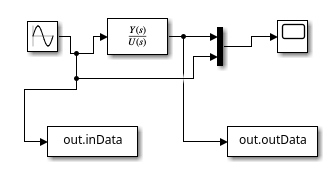
\includegraphics[width=0.8\textwidth]{simulinkOpenModel.png}
\end{figure}

Then I ran the simulation and plotted the results as you can see below:

\begin{figure}[H]
    \centering
    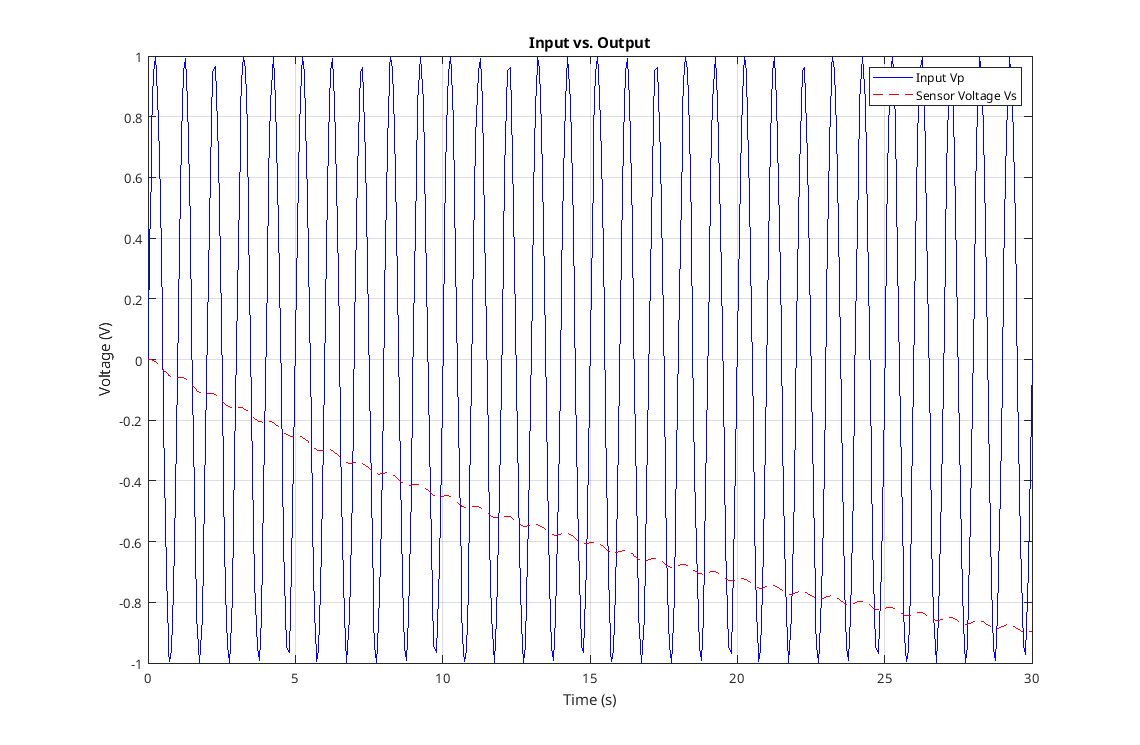
\includegraphics[width=\textwidth]{openPlot.png}
\end{figure}

As for whether the output follows the input I would say in one sense it does, the oscillations match up.
When the input goes down so does the output at the same time.
However, in another sense the output doesn't really follow the input, it does small oscillations but mostly just slowly converges to -1.

\section*{3.}

\textit{
    "[10pts] Derive the closed loop transfer function between reference angle
    $\Theta_R$ and load shaft angle $\Theta_L$ when the controller has a 
    proportional-plus-derivative (PD) control law, i.e.
    $V_P = G_P(\Theta_R - \Theta_L) + G_D\frac{d}{dt}(\Theta_R - \Theta_L).$
    Determine the DC gain of the closed loop system."
}



\end{document}